% !TEX root = ../main.tex

As explained, ERC20 tokens are technically standardized version of smart contracts that could be vulnerable to security flaws. Some of these vulnerabilities have been already discovered and addressed by Ethereum community. One of these issues that is known as "Multiple Withdrawal Attack" was originally opened on GitHub\cite{MikVlad} and raised as separate thread\cite{TomHale} for making it easy to follow. It is security issue in protocol-level and originating from definition of APIs in ERC20 standard for approving and transferring tokens. There are two functions (see figure~\ref{fig:mwaapi}) that can be used to authorize a third party to transfer tokens on behalf of someone else. Using these functions (i.e., \texttt{approve} and \texttt{transferFrom}) in an undesirable situation could result in conditions that allow attacker to transfer more tokens than the owner ever wanted. Since this security issues is at protocol-level, it is important to consider it when implementing a secure ERC20 code. If the token become valuable (e.g., MKR\footnote{\url{https://makerdao.com/en/}, [Accessed online: July 27, 2019]} at \$580 and XIN\footnote{\url{https://mixin.one/}, [Accessed online: July 27, 2019]} at \$210), it may incentivize attackers to use this vulnerability to transfer more token than ever approved.

\begin{figure}[t]
	\centering
	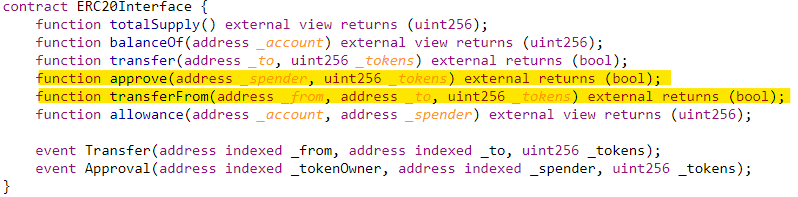
\includegraphics[width=1.0\linewidth]{figures/img14.png}
	\caption{Vulnerable methods in ERC20 API that allow an attacker to withdraw multiple times from approver token pot.}
	\label{fig:mwaapi}
\end{figure}

\subsubsection{Attack analysis}
By using this vulnerability and in existence of race condition\footnote{Execution of two transactions at the same time with undesirable situation.} or front-running\footnote{A course of action where an entity benefits from prior access to privileged market information	about upcoming transactions and trades\cite{eskandari2019sok}.}, an attacker is able to transfer more tokens than approved. This is possible by executing \texttt{transferFrom} function two times, before and after the \texttt{approve} method. According to ERC20 API definition\cite{ERC20Std}:
\begin{enumerate}
	\item \texttt{approve} function allows \texttt{\_spender} to withdraw up to the \texttt{\_value} amount of tokens from token pool of the approver. If this function is called again, it has to overwrites the current allowance with the new \texttt{\_value}.
	\item \texttt{transferFrom} function grants required rights to the spender (account, wallet or other smart contracts) for transferring \texttt{\_value} amount of tokens from address \texttt{\_from} to address \texttt{\_to}.
\end{enumerate}
An attacker can take advantage of the gap between execution of \texttt{approve} and \texttt{transferFrom} functions since the \texttt{approve} method overrides current allowance regardless of whether spender already transferred any tokens or not. Transferred tokens are not trackable and only \texttt{Transfer} event will be logged (which is not sufficient in case of transferring tokens to a third parity). To make it more clear, a possible attack scenario could happen in the below sequences (see figure~\ref{fig:mwaseq}):
\begin{enumerate}
	\item Alice allows Bob to transfer N tokens from her token pool by calling \texttt{approve(Bob, N)}.
	\item After a while, Alice decides to change Bob's approval from N to M by executing \texttt{approve(Bob, M)}.
	\item Bob notices Alice’s second transaction before it was mined and quickly sends another transaction that runs \texttt{transferFrom(Alice, Bob, N)}. This will transfer N Alice’s tokens to Bob.
	\item Bob’s transaction is executed before Alice’s transaction (because of higher transaction fee, miner’s policy or other prioritization techniques) and Bob front-runs Alice’s transaction.
	\item Alice’s transaction is executed after Bob’s and allows Bob to transfer more M tokens.
	\item Bob successfully transferred N Alice’s tokens earlier and gains ability of transferring another M tokens.
	\item Before Alice notices that something went wrong, Bob calls \texttt{transferFrom} method for the second time and transfers M Alice’s tokens by executing \texttt{transferFrom(Alice, Bob, M)}.
\end{enumerate}

In fact, Alice attempted to change Bob’s allowance from N to M, but she made it possible for Bob to transfer N+M of her tokens at most, while Alice never wanted to allow so many transfers to be occurred by Bob. It should be noted that the assumption here is to prevent Bob from withdrawing Alice’s tokens multiple times when allowance changes from N to M. If Bob could withdraw N tokens after initial approval of Alice, this would be considered as a legitimate transfer (since Alice has already approved it). In other words, it would be responsibility of Alice to make sure before approving anything to Bob. After approval, Bob is allowed to transfer up to N tokens even right before allowance change. In figure~\ref{fig:mwaseq}, transaction \#4 would be considered as multiple withdrawal attack since Bob is able to move more M tokens in addition to already transferred N tokens in step \#3. An effective solution must prevent transaction \#4 to prevent Bob from withdrawing multiple times.

\begin{figure}[t]
	\centering
	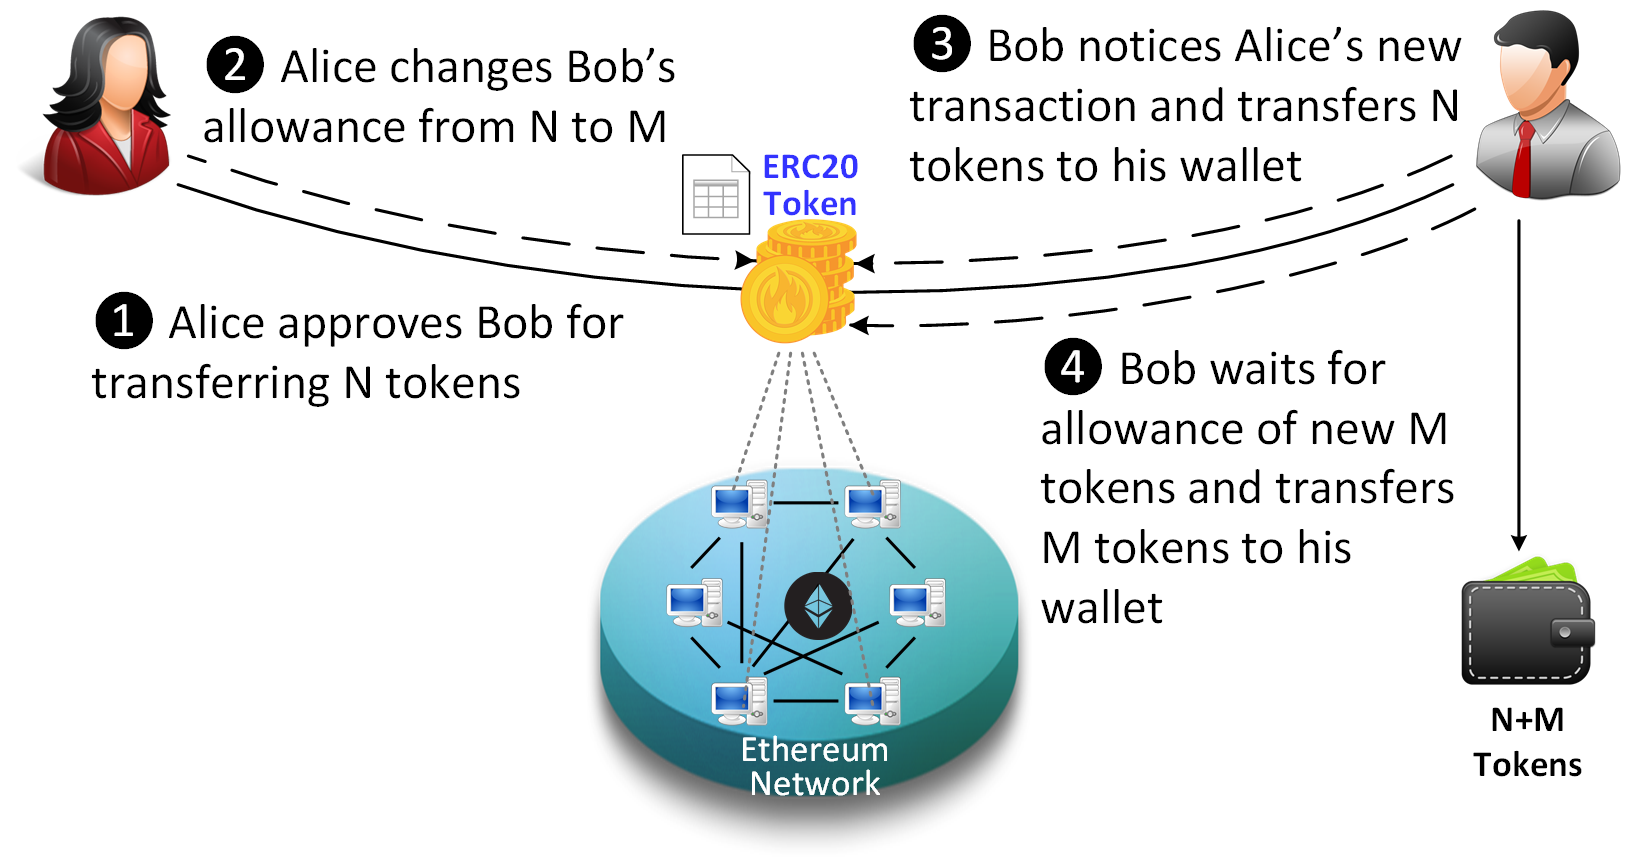
\includegraphics[width=0.8\linewidth]{figures/img13.png}
	\caption{Possible multiple withdrawal attack in ERC20 tokens when Alice changes Bob's allowance from N to M. By front-running, Bob is able to move N+M tokens from Alice's pot.}
	\label{fig:mwaseq}
\end{figure}

\subsubsection{Reproducing the attack}
This attack can be categorized as medium severity since executing it requires tracking of Ethereum transactions and ideally being as a miner. However similar attacks happened before \cite{eskandari2019sok}, \cite{ERC20MWA}. Status.im\footnote{An open source mobile DApp browser and messenger built for Ethereum} was targeted by this attack on June 2017 and miners were able to prioritize purchasing of this token during initial coin offering (ICO)\footnote{When a cryptocurrency startup firm raises money by offering a portion of ownership stake as tokens}. Another similar attack was due to Re-entrancy attack (see section~\ref{sect:reentrancy}) which a potential race condition failed DAO to correctly update the contract state and allowed for funds to be stolen. This shows that feasibility of using similar techniques to execute multiple withdrawal attack.

\subsubsection{Attack mitigation}
As explained in \cite{ERC20MWA} this attack can be mitigated in three levels:
\begin{enumerate}
	\item \textbf{Prevention by token holder:} This approach is recommended by ERC20 standard \cite{ERC20Std} and advises token holders to use user interface (UI) that changes spender allowance from N to 0 and then from 0 to M (instead of set it directly from N to M). Changing allowance to non-zero values after setting to zero will not prevent the attack since the owner would not be able to distinguish how the allowance was set to zero. Was it because of previous \texttt{approve} transaction for changing allowance from N to 0?, Or it was set to 0 by \texttt{transferFrom} method due to token transfers? Although it would be possible to track transferred token through \texttt{Transfer} events, tracking of tokens would not be easy in case of transferring to a third-party. For example, if Alice allows Bob and then Bob transfers tokens to Carole, \texttt{Transfer} event creates a log showing Carole moved tokens from Alice. Despite recommendation of this approach by ERC20 standard, we will not use it in our proposal since it is not distinguishable which transaction (i.e., owner or attacker transaction) has set allowance to zero. However, it might be considered as last resort for already deployed ERC20 tokens, but for new deployments (focus of this project), prevention in the contract is more efficient (and sustainable) than UI.

	\item \textbf{Prevention by \texttt{approve} method:} In this approach, \texttt{approve} method changes spender allowance from N to M atomically by comparing new allowance with transferred tokens and set it accordingly. Although this is promising approach, but setting new allowance in \texttt{approve} method must satisfy ERC20 constraint that says "If this function is called again it overwrites the current allowance with \texttt{\_value}" \cite{ERC20Std}. In other words, any adjustments in allowance is prohibited which makes the \texttt{approve} method vulnerable. For example, considering front-running by Bob when Alice wants to change Bob allowance form 100 to 110, the \texttt{approve} method can reveal 100 transferred tokens by Bob. However, based on ERC20 constraints, it must not adjust new allowance to 110-100=10, it has to set it literally to 110, which is allowing Bob for transferring 100+110=210 tokens in total. Overall, securing \texttt{approve} method can not prevent the attack while adhering constraints of the ERC20 standard. Therefore, we will not use this approach in our proposal.

	\item \textbf{Prevention by \texttt{transferFrom} method:} Based on ERC20 constraint, "approve functions allows \texttt{\_spender} to withdraw from your account multiple times, up to the \texttt{\_value}". Hence, spender must not be able to transfer more than authorized tokens. That being said, \texttt{transferFrom} method can be secured in a way that prevents M new tokens transfer in case of already transferred N tokens. By comparing transferred tokens in \texttt{transferFrom} method, spender will be restricted to move solely remained tokens of his allowance. In case of trying to transfer more tokens than allowed, the transaction fails. For example, Alice's new transaction for increasing Bob allowance from 100 to 110, sets Bob allowance to 110 (since the \texttt{approve} method does not adjust allowance). However, \texttt{transferFrom} method does not allow Bob from transferring more than 10 tokens if he had already transferred 100 tokens. This approach  mitigates the attack by adding a piece of code to the \texttt{transferFrom} method (see figure~\ref{fig:mwapre}).
\end{enumerate}

\begin{figure}[t]
	\centering
	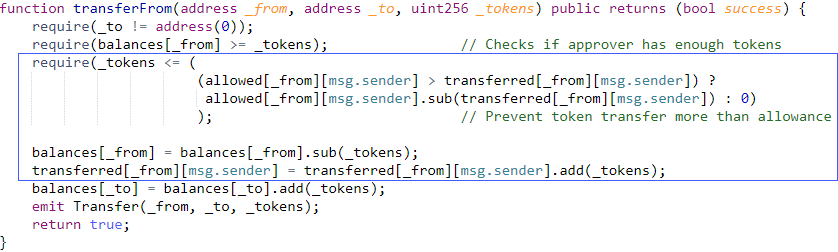
\includegraphics[width=0.9\linewidth]{figures/img15.png}
	\caption{Added code to \texttt{transferFrom} method to prevent more token transfer than allowed. It uses a new mapping variable to track transferred tokens by each spender. }
	\label{fig:mwapre}
\end{figure}

Overall, if token holders approve someone to transfer $N$ tokens, the spender can transfer exactly $N$ tokens, even if they change it afterwards. This is considered a legitimate transaction and responsibility of the approver before allowing any token transfer. An attack can happen when changing allowance from $N$ to $M$, that allows spender to transfer $N+M$ tokens. This attack can happen in case of front-running (or existence of race condition) by the approved side. As evaluated in \cite{ERC20MWA}, preventing the attack in \texttt{transferFrom} function is more compatible approach than \texttt{approve} method. Although it consumes more Gas\footnote{Internal pricing for running transactions in Ethereum. It prevent infinite use of computing resources.}, we will use it in our proposal for having more secure ERC20 token.